\documentclass[twoside]{book}

% Packages required by doxygen
\usepackage{fixltx2e}
\usepackage{calc}
\usepackage{doxygen}
\usepackage[export]{adjustbox} % also loads graphicx
\usepackage{graphicx}
\usepackage[utf8]{inputenc}
\usepackage{makeidx}
\usepackage{multicol}
\usepackage{multirow}
\PassOptionsToPackage{warn}{textcomp}
\usepackage{textcomp}
\usepackage[nointegrals]{wasysym}
\usepackage[table]{xcolor}

% Font selection
\usepackage[T1]{fontenc}
\usepackage[scaled=.90]{helvet}
\usepackage{courier}
\usepackage{amssymb}
\usepackage{sectsty}
\renewcommand{\familydefault}{\sfdefault}
\allsectionsfont{%
  \fontseries{bc}\selectfont%
  \color{darkgray}%
}
\renewcommand{\DoxyLabelFont}{%
  \fontseries{bc}\selectfont%
  \color{darkgray}%
}
\newcommand{\+}{\discretionary{\mbox{\scriptsize$\hookleftarrow$}}{}{}}

% Page & text layout
\usepackage{geometry}
\geometry{%
  a4paper,%
  top=2.5cm,%
  bottom=2.5cm,%
  left=2.5cm,%
  right=2.5cm%
}
\tolerance=750
\hfuzz=15pt
\hbadness=750
\setlength{\emergencystretch}{15pt}
\setlength{\parindent}{0cm}
\setlength{\parskip}{3ex plus 2ex minus 2ex}
\makeatletter
\renewcommand{\paragraph}{%
  \@startsection{paragraph}{4}{0ex}{-1.0ex}{1.0ex}{%
    \normalfont\normalsize\bfseries\SS@parafont%
  }%
}
\renewcommand{\subparagraph}{%
  \@startsection{subparagraph}{5}{0ex}{-1.0ex}{1.0ex}{%
    \normalfont\normalsize\bfseries\SS@subparafont%
  }%
}
\makeatother

% Headers & footers
\usepackage{fancyhdr}
\pagestyle{fancyplain}
\fancyhead[LE]{\fancyplain{}{\bfseries\thepage}}
\fancyhead[CE]{\fancyplain{}{}}
\fancyhead[RE]{\fancyplain{}{\bfseries\leftmark}}
\fancyhead[LO]{\fancyplain{}{\bfseries\rightmark}}
\fancyhead[CO]{\fancyplain{}{}}
\fancyhead[RO]{\fancyplain{}{\bfseries\thepage}}
\fancyfoot[LE]{\fancyplain{}{}}
\fancyfoot[CE]{\fancyplain{}{}}
\fancyfoot[RE]{\fancyplain{}{\bfseries\scriptsize Generated by Doxygen }}
\fancyfoot[LO]{\fancyplain{}{\bfseries\scriptsize Generated by Doxygen }}
\fancyfoot[CO]{\fancyplain{}{}}
\fancyfoot[RO]{\fancyplain{}{}}
\renewcommand{\footrulewidth}{0.4pt}
\renewcommand{\chaptermark}[1]{%
  \markboth{#1}{}%
}
\renewcommand{\sectionmark}[1]{%
  \markright{\thesection\ #1}%
}

% Indices & bibliography
\usepackage{natbib}
\usepackage[titles]{tocloft}
\setcounter{tocdepth}{3}
\setcounter{secnumdepth}{5}
\makeindex

% Hyperlinks (required, but should be loaded last)
\usepackage{ifpdf}
\ifpdf
  \usepackage[pdftex,pagebackref=true]{hyperref}
\else
  \usepackage[ps2pdf,pagebackref=true]{hyperref}
\fi
\hypersetup{%
  colorlinks=true,%
  linkcolor=blue,%
  citecolor=blue,%
  unicode%
}

% Custom commands
\newcommand{\clearemptydoublepage}{%
  \newpage{\pagestyle{empty}\cleardoublepage}%
}

\usepackage{caption}
\captionsetup{labelsep=space,justification=centering,font={bf},singlelinecheck=off,skip=4pt,position=top}

%===== C O N T E N T S =====

\begin{document}

% Titlepage & ToC
\hypersetup{pageanchor=false,
             bookmarksnumbered=true,
             pdfencoding=unicode
            }
\pagenumbering{alph}
\begin{titlepage}
\vspace*{7cm}
\begin{center}%
{\Large My Project }\\
\vspace*{1cm}
{\large Generated by Doxygen 1.8.13}\\
\end{center}
\end{titlepage}
\clearemptydoublepage
\pagenumbering{roman}
\tableofcontents
\clearemptydoublepage
\pagenumbering{arabic}
\hypersetup{pageanchor=true}

%--- Begin generated contents ---
\chapter{File Index}
\section{File List}
Here is a list of all documented files with brief descriptions\+:\begin{DoxyCompactList}
\item\contentsline{section}{\hyperlink{main_8cpp}{main.\+cpp} \\*Driver program for the project, exposes an H\+T\+TP server on port 8080 to handle A\+PI requests }{\pageref{main_8cpp}}{}
\end{DoxyCompactList}

\chapter{File Documentation}
\hypertarget{main_8cpp}{}\section{main.\+cpp File Reference}
\label{main_8cpp}\index{main.\+cpp@{main.\+cpp}}


Driver program for the project, exposes an H\+T\+TP server on port 8080 to handle A\+PI requests.  


{\ttfamily \#include $<$set$>$}\newline
{\ttfamily \#include $<$cstdio$>$}\newline
{\ttfamily \#include $<$string$>$}\newline
{\ttfamily \#include $<$stdexcept$>$}\newline
{\ttfamily \#include \char`\"{}device.\+hpp\char`\"{}}\newline
{\ttfamily \#include \char`\"{}mqtt\+\_\+subscriber.\+hpp\char`\"{}}\newline
Include dependency graph for main.\+cpp\+:
\nopagebreak
\begin{figure}[H]
\begin{center}
\leavevmode
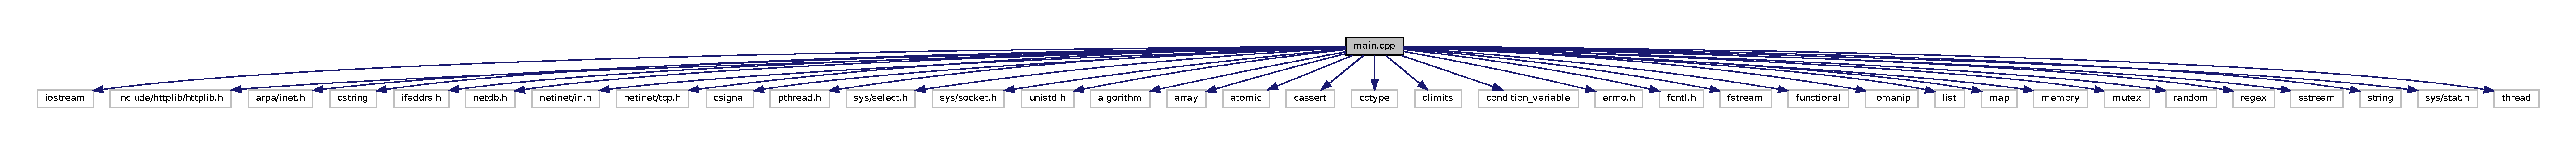
\includegraphics[width=350pt]{main_8cpp__incl}
\end{center}
\end{figure}
\subsection*{Macros}
\begin{DoxyCompactItemize}
\item 
\mbox{\Hypertarget{main_8cpp_a70bb99d4d6c2e1a35c26a6c84222be7f}\label{main_8cpp_a70bb99d4d6c2e1a35c26a6c84222be7f}} 
\#define {\bfseries I\+N\+P\+U\+T\+\_\+\+K\+EY}~\char`\"{}input\char`\"{}
\item 
\mbox{\Hypertarget{main_8cpp_aaf1329031adc4fd484b6edc8abfd7434}\label{main_8cpp_aaf1329031adc4fd484b6edc8abfd7434}} 
\#define {\bfseries I\+N\+P\+U\+T\+\_\+\+T\+Y\+P\+E\+\_\+\+K\+EY}~\char`\"{}input\+\_\+type\char`\"{}
\item 
\mbox{\Hypertarget{main_8cpp_af2685dfc271d06adb84a0d94a31d0de3}\label{main_8cpp_af2685dfc271d06adb84a0d94a31d0de3}} 
\#define {\bfseries I\+N\+P\+U\+T\+\_\+\+S\+E\+T\+T\+I\+N\+G\+S\+\_\+\+K\+EY}~\char`\"{}input\+\_\+settings\char`\"{}
\item 
\mbox{\Hypertarget{main_8cpp_a35c11f02aa6db89430334483bd425831}\label{main_8cpp_a35c11f02aa6db89430334483bd425831}} 
\#define {\bfseries O\+U\+T\+P\+U\+T\+\_\+\+E\+R\+R\+O\+R\+\_\+\+K\+EY}~\char`\"{}error\char`\"{}
\item 
\mbox{\Hypertarget{main_8cpp_a6bb3b62d951dfd91bb84d00c6d4580ea}\label{main_8cpp_a6bb3b62d951dfd91bb84d00c6d4580ea}} 
\#define {\bfseries O\+U\+T\+P\+U\+T\+\_\+\+V\+A\+L\+I\+D\+\_\+\+K\+EY}~\char`\"{}valid\+\_\+request\char`\"{}
\item 
\mbox{\Hypertarget{main_8cpp_a3cdc10e08bf545f186ce9ddc0f347dc0}\label{main_8cpp_a3cdc10e08bf545f186ce9ddc0f347dc0}} 
\#define {\bfseries I\+N\+V\+A\+L\+I\+D\+\_\+\+R\+E\+Q\+U\+E\+S\+T\+\_\+\+B\+O\+DY}~\char`\"{}invalid\+\_\+request\char`\"{}
\item 
\mbox{\Hypertarget{main_8cpp_a20ec364faebf30a95ab7d9cad53f1f24}\label{main_8cpp_a20ec364faebf30a95ab7d9cad53f1f24}} 
\#define {\bfseries B\+A\+D\+\_\+\+R\+E\+Q\+U\+E\+S\+T\+\_\+\+J\+S\+ON}~\char`\"{}request format isn\textquotesingle{}t correct\char`\"{}
\end{DoxyCompactItemize}
\subsection*{Functions}
\begin{DoxyCompactItemize}
\item 
int \hyperlink{main_8cpp_a840291bc02cba5474a4cb46a9b9566fe}{main} (void)
\begin{DoxyCompactList}\small\item\em Main driver function of the program, runs an H\+T\+TP server on port 8080 to process incoming requests (blocking!) \end{DoxyCompactList}\end{DoxyCompactItemize}
\subsection*{Variables}
\begin{DoxyCompactItemize}
\item 
const std\+::set$<$ std\+::string $>$ {\bfseries Input\+Type}
\end{DoxyCompactItemize}


\subsection{Detailed Description}
Driver program for the project, exposes an H\+T\+TP server on port 8080 to handle A\+PI requests. 



\subsection{Function Documentation}
\mbox{\Hypertarget{main_8cpp_a840291bc02cba5474a4cb46a9b9566fe}\label{main_8cpp_a840291bc02cba5474a4cb46a9b9566fe}} 
\index{main.\+cpp@{main.\+cpp}!main@{main}}
\index{main@{main}!main.\+cpp@{main.\+cpp}}
\subsubsection{\texorpdfstring{main()}{main()}}
{\footnotesize\ttfamily int main (\begin{DoxyParamCaption}\item[{void}]{ }\end{DoxyParamCaption})}



Main driver function of the program, runs an H\+T\+TP server on port 8080 to process incoming requests (blocking!) 

\begin{DoxyReturn}{Returns}
int -\/ status code 
\end{DoxyReturn}


\subsection{Variable Documentation}
\mbox{\Hypertarget{main_8cpp_a0320ad1b70d522baab095239e6454546}\label{main_8cpp_a0320ad1b70d522baab095239e6454546}} 
\index{main.\+cpp@{main.\+cpp}!Input\+Type@{Input\+Type}}
\index{Input\+Type@{Input\+Type}!main.\+cpp@{main.\+cpp}}
\subsubsection{\texorpdfstring{Input\+Type}{InputType}}
{\footnotesize\ttfamily const std\+::set$<$std\+::string$>$ Input\+Type}

{\bfseries Initial value\+:}
\begin{DoxyCode}
= \{
    \textcolor{stringliteral}{"UserManualInput"},
    \textcolor{stringliteral}{"DisplayInput"},
    \textcolor{stringliteral}{"MusicInput"},
    \textcolor{stringliteral}{"WeatherInput"},
    \textcolor{stringliteral}{"BrightnessInput"},
    \textcolor{stringliteral}{"RandomInput"}\}
\end{DoxyCode}

%--- End generated contents ---

% Index
\backmatter
\newpage
\phantomsection
\clearemptydoublepage
\addcontentsline{toc}{chapter}{Index}
\printindex

\end{document}
